%%%%%%%%%%%%%%%%%%%%% PACKAGE IMPORTS %%%%%%%%%%%%%%%%%%%%%
\documentclass{article}
\usepackage{import}
\subimport*{./}{macro}

\usepackage{amsmath, amsfonts, amsthm, amssymb}
\usepackage{lmodern}
\usepackage{microtype}
\usepackage{fullpage}       
\usepackage{changepage}
\usepackage{hyperref}
\usepackage{blindtext}
\usepackage{subcaption}
\hypersetup{
    colorlinks=true,
    linkcolor=blue,
    filecolor=magenta,      
    urlcolor=blue,
    pdftitle={Overleaf Example},
    pdfpagemode=FullScreen,
    }
\urlstyle{same}

\newenvironment{level}%
{\addtolength{\itemindent}{2em}}%
{\addtolength{\itemindent}{-2em}}

\usepackage{amsmath,amsthm,amssymb}

\usepackage[nooldvoltagedirection]{circuitikz}
\usetikzlibrary{decorations,arrows,shapes}

\usepackage{datetime}
\usepackage{etoolbox}
\usepackage{enumerate}
\usepackage{enumitem}
\usepackage{listings}
\usepackage{array}
\usepackage{varwidth}
\usepackage{tcolorbox}
\usepackage{amsmath}
\usepackage{circuitikz}
\usepackage{verbatim}
\usepackage[linguistics]{forest}
\usepackage{listings}
\usepackage{xcolor}
\renewcommand{\rmdefault}{cmss}


\newcommand\doubleplus{+\kern-1.3ex+\kern0.8ex}
\newcommand\mdoubleplus{\ensuremath{\mathbin{+\mkern-10mu+}}}

\definecolor{codegreen}{rgb}{0,0.6,0}
\definecolor{codegray}{rgb}{0.5,0.5,0.5}
\definecolor{codepurple}{rgb}{0.58,0,0.82}
\definecolor{backcolour}{rgb}{0.95,0.95,0.92}

\lstdefinestyle{mystyle}{
    language=Python,
    basicstyle=\ttfamily\small,
    keywordstyle=\color{blue},
    stringstyle=\color{red},
    commentstyle=\color{green},
    morecomment=[l][\color{magenta}]{\#},
    backgroundcolor=\color{backcolour},   
    breakatwhitespace=false,         
    breaklines=true,                 
    captionpos=b,                    
    keepspaces=true,                 
    numbers=left,                    
    numbersep=5pt,                  
    showspaces=false,                
    showstringspaces=false,
    showtabs=false,                  
    tabsize=2
}

\lstset{style=mystyle}
\setlength{\parindent}{0pt}
\setlength{\parskip}{5pt plus 1pt}

\providetoggle{questionnumbers}
\settoggle{questionnumbers}{true}
\newcommand{\noquestionnumbers}{
    \settoggle{questionnumbers}{false}
}

\newcounter{questionCounter}
\newenvironment{question}[2][\arabic{questionCounter}]{%
    \ifnum\value{questionCounter}=0 \else {\newpage}\fi%
    \setcounter{partCounter}{0}%
    \vspace{.25in} \hrule \vspace{0.5em}%
    \noindent{\bf \iftoggle{questionnumbers}{Question #1: }{}#2}%
    \addtocounter{questionCounter}{1}%
    \vspace{0.8em} \hrule \vspace{.10in}%
}

\newcounter{partCounter}[questionCounter]
\renewenvironment{part}[1][\alph{partCounter}]{%
    \addtocounter{partCounter}{1}%
    \vspace{.10in}%
    \begin{indented}%
       {\bf (#1)} %
}{\end{indented}}

\def\indented#1{\list{}{}\item[]}
\let\indented=\endlist
\def\show#1{\ifdefempty{#1}{}{#1\\}}
\def\IMP{\longrightarrow}
\def\AND{\wedge}
\def\OR{\vee}
\def\BI{\leftrightarrow}
\def\DIFF{\setminus}
\def\SUB{\subseteq}


\newcolumntype{C}{>{\centering\arraybackslash}m{1.5cm}}
\renewcommand\qedsymbol{$\blacksquare$}
\newtcolorbox{answer}
{
  colback   = green!5!white,    % Background colorucyitc,
  colframe  = green!75!black,   % Outline color
  box align = center,           % Align box on text line
  varwidth upper,               % Enables multi line input
  hbox                          % Bounds box to text width
}

\newcommand{\myhwname}{CSE 446 Homework 3}
\newcommand{\myname}{Sebastian Liu}
\newcommand{\myemail}{ll57@cs.washington.edu}
\newcommand{\mysection}{AB}
\newcommand{\dollararrow}{\stackrel{\$}{\leftarrow}}
%%%%%%%%%%%%%%%%%%%%%%%%%%%%%%%%%%%%%%%%%%%%%%%%%%%%%%%%%%%

%%%%%%%%%%%%%%%%%%% Document Options %%%%%%%%%%%%%%%%%%%%%%
\noquestionnumbers
%%%%%%%%%%%%%%%%%%%%%%%%%%%%%%%%%%%%%%%%%%%%%%%%%%%%%%%%%%%

%%%%%%%%%%%%%%%%%%%%%%%% WORK BELOW %%%%%%%%%%%%%%%%%%%%%%%%
\begin{document}

\begin{center}
    \textbf{Homework 3} \bigskip
\end{center}

%%%%%%%%%%%%%%%%%%%%%%%% Task 1 %%%%%%%%%%%%%%%%%%%%%%%%M
\begin{question}{A1.}
     \begin{part}
        \begin{answer}
            False. Neural networks are non-convex, and for large networks, gradient decent can blow up or go to zero.
        \end{answer}
     \end{part}

     \begin{part}
        \begin{answer}
            False. Initializing all weights to zero can cause all the neurons on the same layer to have the same weights and receive the same gradients
            updates, which is not ideal since we want the neurons to learn different features from the input.
        \end{answer}
     \end{part}

     \begin{part}
        \begin{answer}
            True. If we don't have non-linearity, then the network would behave like a linear model regardless of the number of layers, and we
            wouldn't be able to learn complex (non-linear) decision boundaries from the input.
        \end{answer}
     \end{part}

     \begin{part}
        \begin{answer}
            False. If we use a recursive algorithm where we store the intermediate results and errors of the forward pass to use in the backward pass,
            the time complexities of forward and backward passes are roughly the same.
        \end{answer}
     \end{part}

     \begin{part}
        \begin{answer}
            False. The model we choose is dependant on the specific problem, the amount of data, computational resources etc.
            If we have a small dataset with a simple linear relationship, using a simple linear model would potentially produce better results
            than using neural networks where we might easily overfit the data.
        \end{answer}
     \end{part}
\end{question}

%%%%%%%%%%%%%%%%%%%%%%%% Task 2 %%%%%%%%%%%%%%%%%%%%%%%%
\begin{question}{A2.}
    \begin{part}
       \begin{answer}
        \begin{align*}
            \phi(x) \cdot \phi(x') &= \sum_{i=0}^{\infty} \left( \frac{1}{\sqrt{i!}} e^{-\frac{x^2}{2}} x^i \right) \left( \frac{1}{\sqrt{i!}} e^{-\frac{x'^2}{2}} x'^i \right)  \\
            &= \sum_{i=0}^{\infty} \frac{1}{i!} e^{-\frac{x^2}{2}} e^{-\frac{x'^2}{2}} x^i x'^i\\
            &= e^{-\frac{x^2}{2}} e^{-\frac{x'^2}{2}} \sum_{i=0}^{\infty} \frac{x^i x'^i}{i!} \\
            &= e^{-\frac{x^2}{2}} e^{-\frac{x'^2}{2}} e^{xx'} \tag{Taylor series expansion of $e^{xx'}$} \\
            &= e^{-\frac{x^2}{2} - \frac{x'^2}{2} + xx'} \\
            &= e^{-\frac{x^2 + x'^2 - 2xx'}{2}} \\
            &= e^{-\frac{(x - x')^2}{2}}
        \end{align*}
        Therefore, $K(x, x') = e^{-\frac{(x - x')^2}{2}}$ is a kernel function for the feature map $\phi$, since we have shown that $\phi(x) \cdot \phi(x') = e^{-\frac{(x - x')^2}{2}} = K(x, x')$.
        \end{answer}
    \end{part}
\end{question}

%%%%%%%%%%%%%%%%%%%%%%%% Task 3 %%%%%%%%%%%%%%%%%%%%%%%%
\begin{question}{A3.}
    \begin{part}
        \begin{answer}
            Grid search, Leave-One-Out cross-validation:
            \begin{itemize}
                \item \textbf{For RBF Kernel:} $\lambda = $ 0.002329951810515372, $\gamma = $ 11.201924992299844 (by the heuristic provided)
                \item \textbf{For Polynomial Kernel:} $\lambda =$ 3.727593720314938e-5, $d = $ 16
            \end{itemize}
        \end{answer}
     \end{part}
 
     \begin{part}
        \begin{answer}
            $\hat{f}_{\text{rbf}}(x)$:\\
            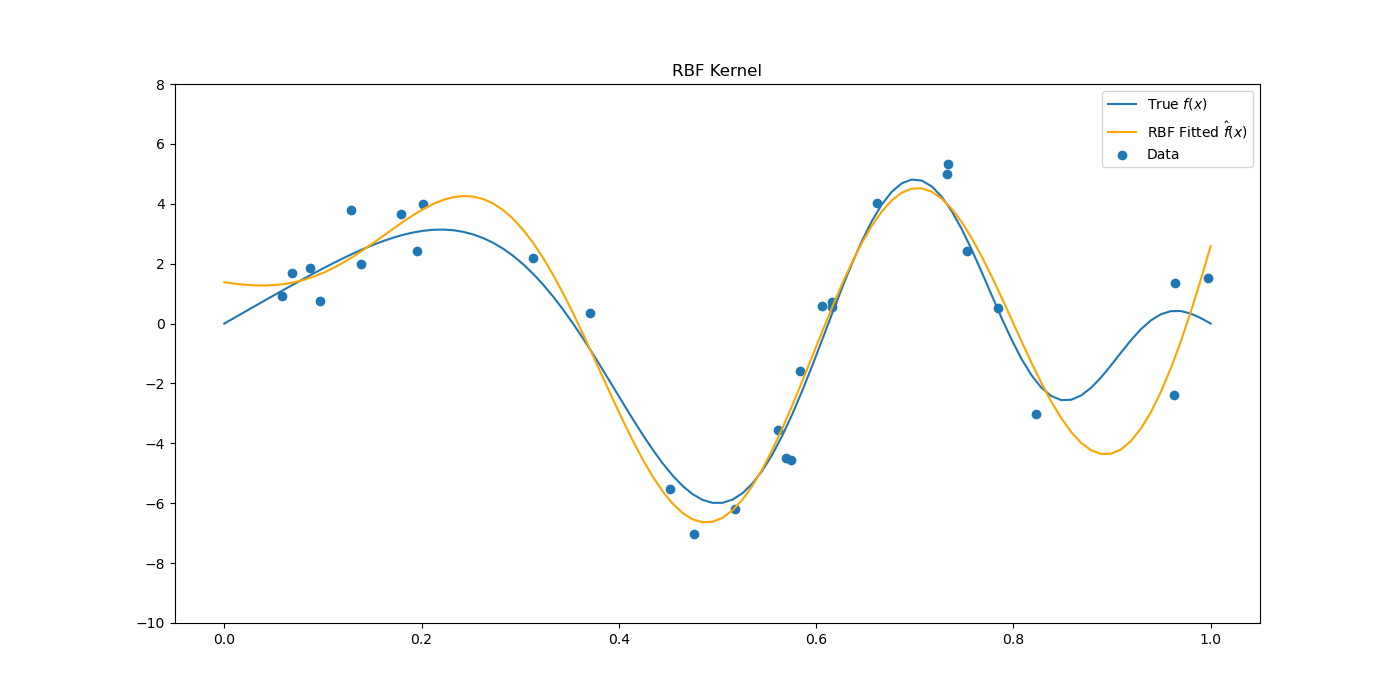
\includegraphics[width=0.895\linewidth]{./rbf.png}\\
            $\hat{f}_{\text{poly}}(x)$:\\
            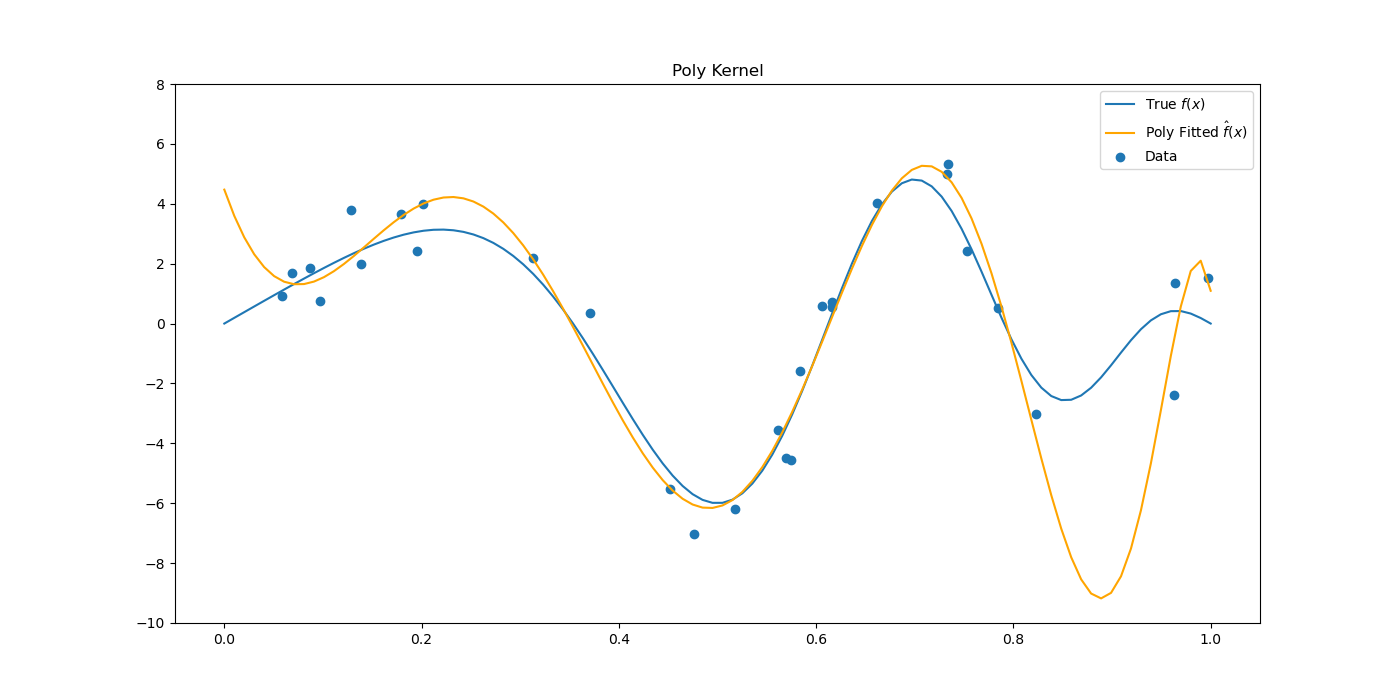
\includegraphics[width=0.895\linewidth]{./poly.png}
        \end{answer}
      \end{part}
\end{question}

%%%%%%%%%%%%%%%%%%%%%%%% Task 4 %%%%%%%%%%%%%%%%%%%%%%%%
\begin{question}{A4.}
     \begin{part}[b]
         \begin{answer}
            Cross-entropy search (Learning rate = 1e-3, Epochs = 30):\\
            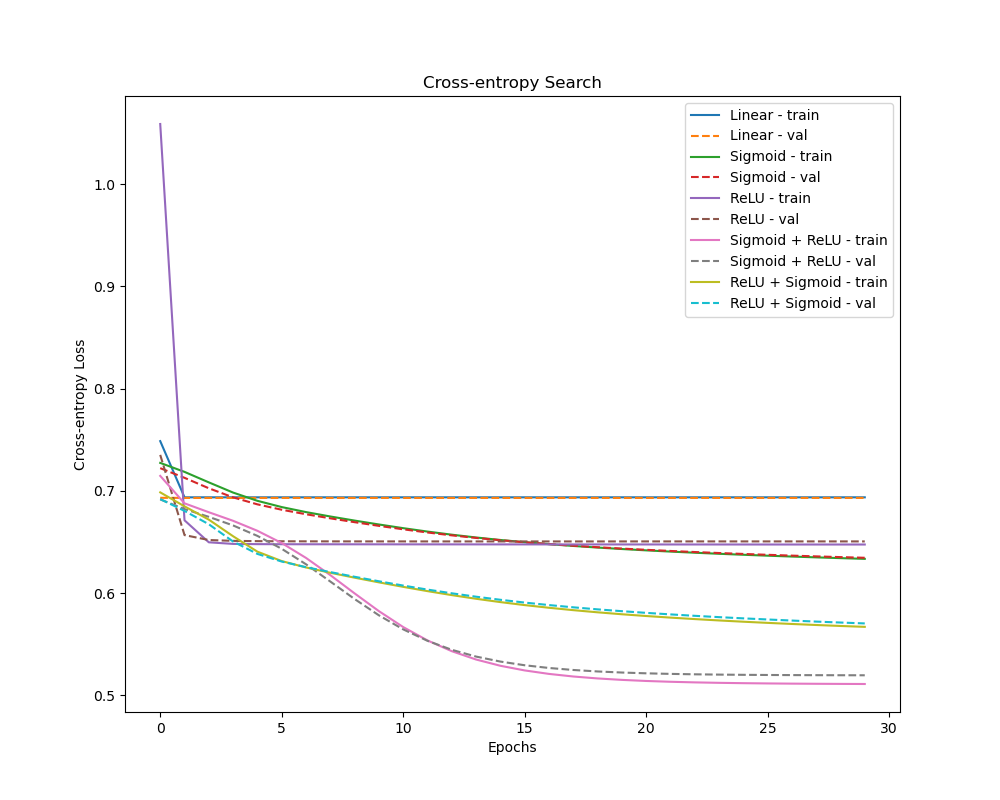
\includegraphics[width=0.722\linewidth]{./ce.png} \\
            Mean Squared Error search (Learning rate = 1e-2, Epochs = 20):\\
            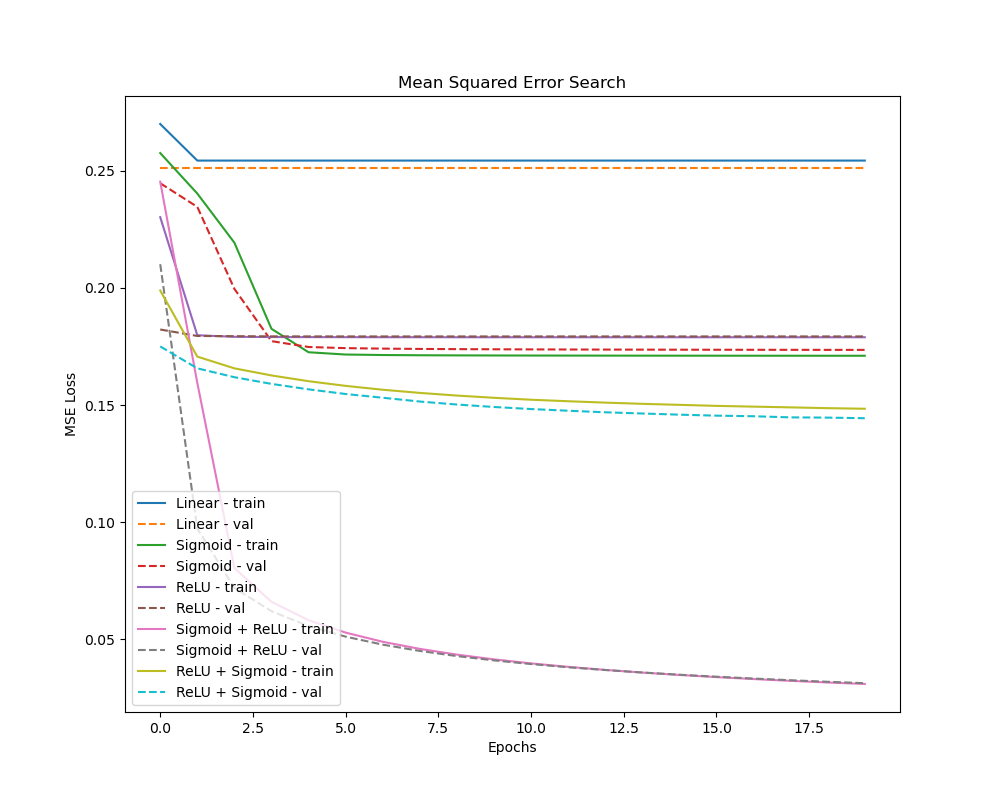
\includegraphics[width=0.722\linewidth]{./mse.png}
          \end{answer}
      \end{part}

      \begin{part}[c]
        \begin{answer}
         \textbf{Best Performing Architecture for Cross-entropy loss:} NN with two hidden layer (each with 2 units) and Sigmoid, ReLU activation functions after first and
         second hidden layers, respectively. \\
            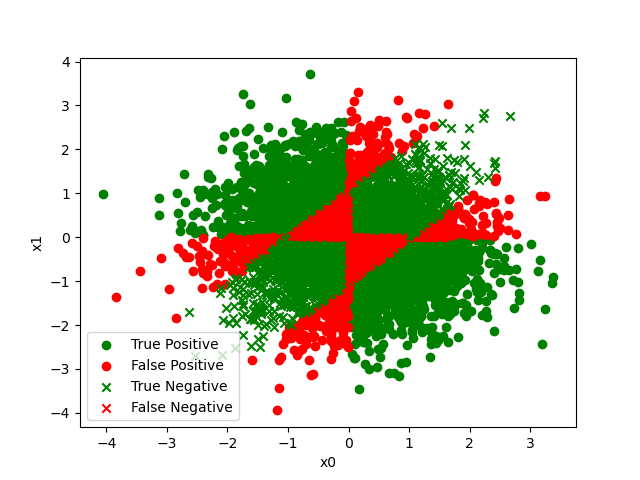
\includegraphics[width=0.722\linewidth]{./ce_scatter.png} \\
        \textbf{Accuracy on test set:} 0.75\\\\
        \textbf{Best Performing Architecture for MSE loss:} NN with two hidden layer (each with 2 units) and Sigmoid, ReLU activation functions after first and
         second hidden layers, respectively. \\
            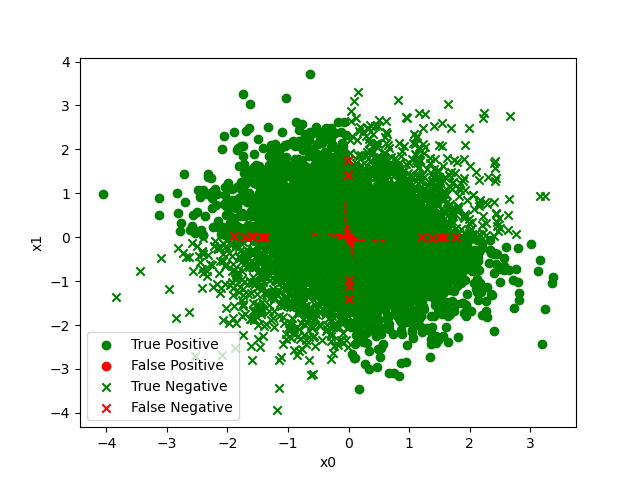
\includegraphics[width=0.722\linewidth]{./mse_scatter.png} \\
        \textbf{Accuracy on test set:} 0.98
        \end{answer}
     \end{part}
 
\end{question}
%%%%%%%%%%%%%%%%%%%%%%%% Task 5 %%%%%%%%%%%%%%%%%%%%%%%%
\begin{question}{A5.}
    \begin{part}
       \begin{answer}
            \textbf{F1}: Test Loss: 0.0829, Test Accuracy: 97.64\% \\
            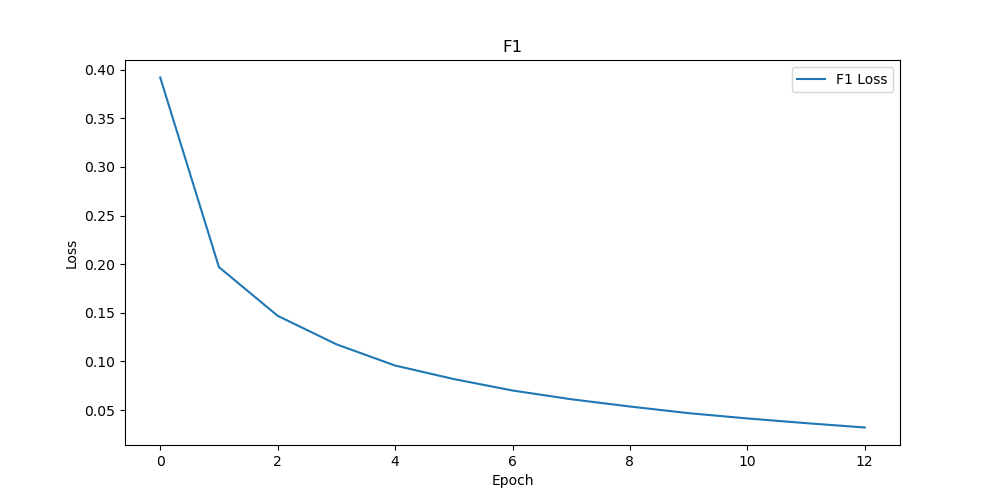
\includegraphics[width=\linewidth]{./f1.png}\\
        \end{answer}
    \end{part}

    \begin{part}
        \begin{answer}
            \textbf{F2}: Test Loss: 0.1482, Test Accuracy: 96.47\% \\
            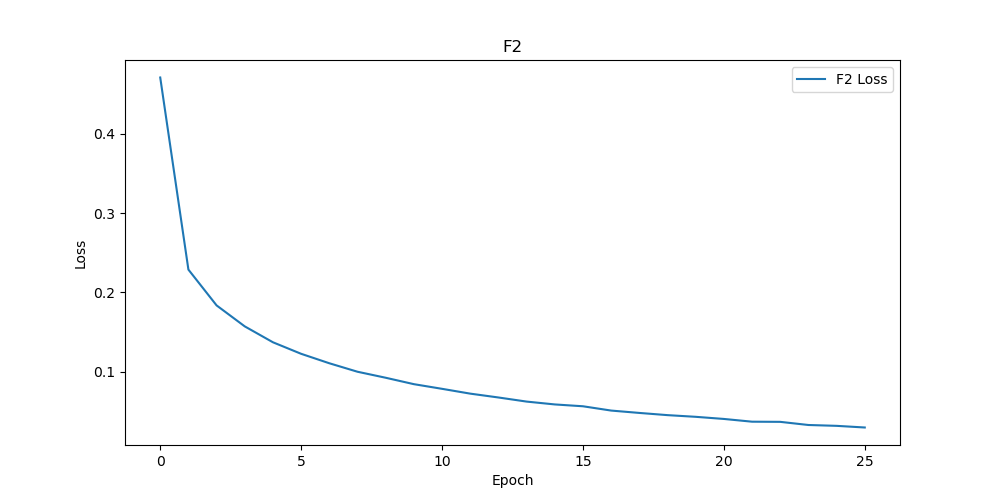
\includegraphics[width=\linewidth]{./f2.png}
         \end{answer}
     \end{part}

     \begin{part}
        \begin{answer}
           \textbf{Number of Parameters in F1:} 50890 \\
            \textbf{Number of Parameters in F2:} 26506 \\

            The F1 network, which is wide and shallow, was more accurate (performed better) than the narrow and deep F2.
            F1 has more parameters giving it higher degrees of flexibility to fit the data, which could be why it learned
            better for this task. Since the MNIST images are relatively simple, having a wider network like F1 seems to be enough
            to recognize the digits well, and making the network deeper (e.g. F2) didn't help as much.
         \end{answer}
     \end{part}
\end{question}
%%%%%%%%%%%%%%%%%%%%%%%% Task 6 %%%%%%%%%%%%%%%%%%%%%%%%
\begin{question}{A6.}
    \begin{part}
       \begin{answer}
            20 hours
        \end{answer}
    \end{part}
\end{question}
\end{document}
